\subsection{Data description}
The training data consists in a matrix Ytrain of size 1774x15082, corresponding to 1774 users 
and 15802 artists. Element r(i,j) expresses how many times user i has listened to the artist j.
If the value is 0, it means we do not have information for that user,artist pair.

We are also given the friendship information in an adjacency matrix.

\subsection{Exploratory Data Analysis}

The listening counts matrix is very sparse with a density of only 0.0026 per cent.
The highest count is 352698.

The average sparsity per user is . The average sparsity per artist is.
A histogram of count, shown in Fig1 tells us that tfollows a heavy tailed distribution.
One method to deal with skewed data is to use the Box-Cox transform :
In our case, we can choose lambda=0 since for us y >0 and y values are very high. 
This transform will make the distances between counts much smaller and will reduce the influence on the error and the model parameters modelling of very high counts.


\begin{figure}[h]
  \centering
  \begin{subfigure}[b]{0.45\textwidth}
   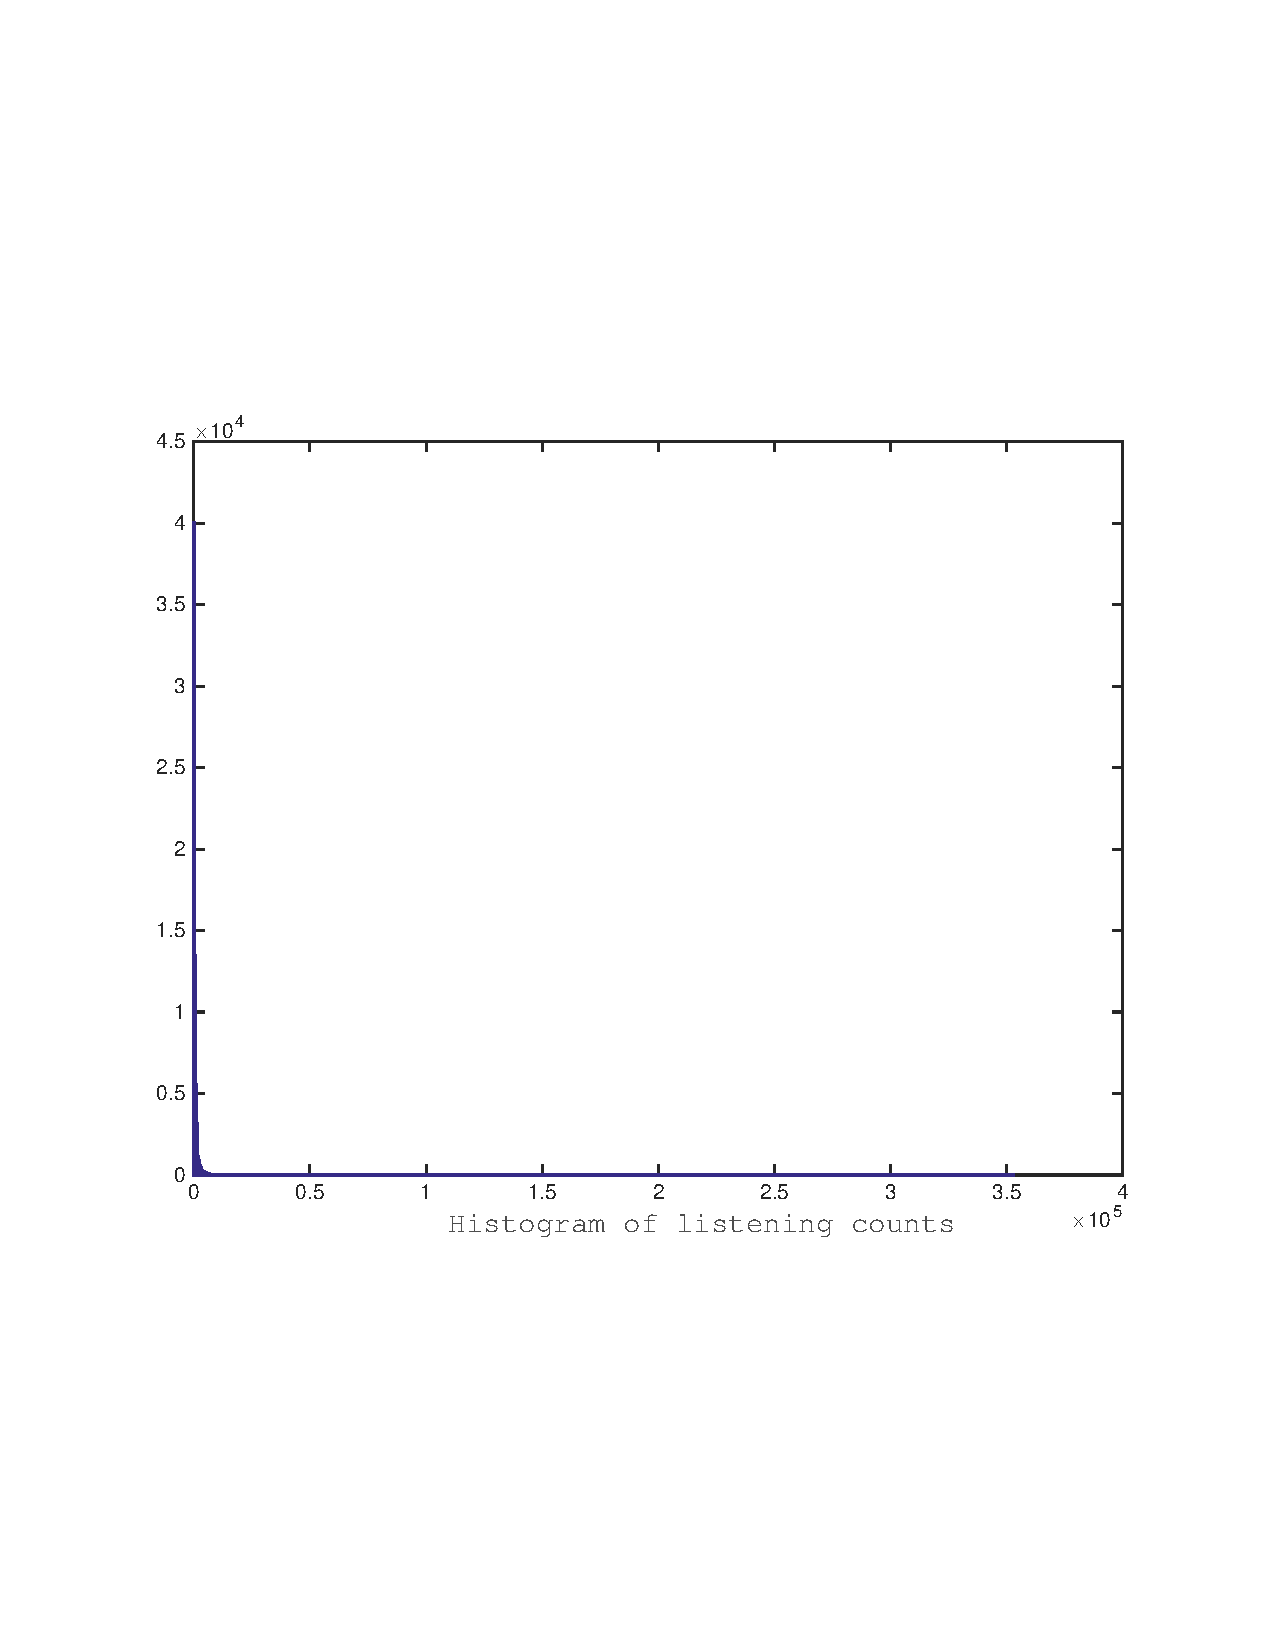
\includegraphics[width=\textwidth]{figures/histYtrain_crop.pdf}
    \caption{Positive Image}
  \end{subfigure}
  \begin{subfigure}[b]{0.45\textwidth}
    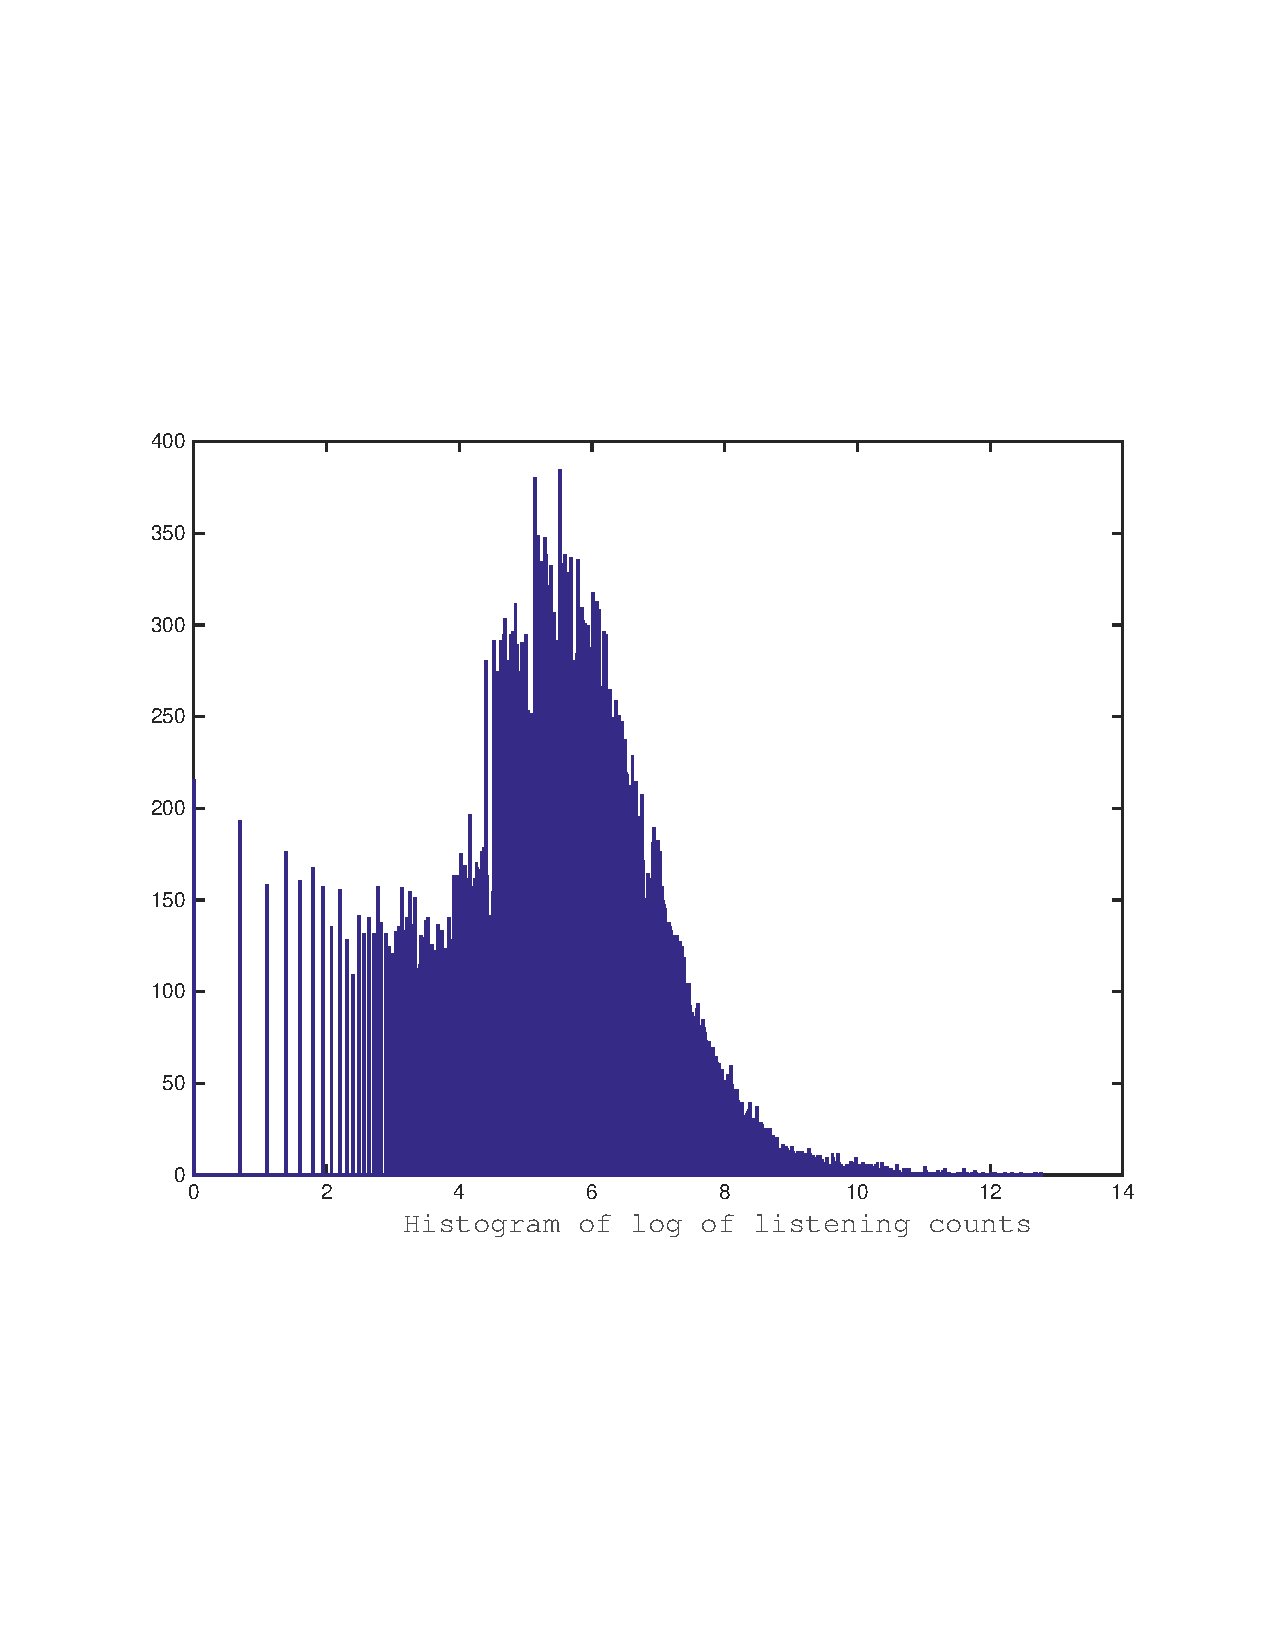
\includegraphics[width=\textwidth]{figures/histLogYtrain_crop.pdf}
    \caption{Negative image.}
  \end{subfigure}
  \caption{Examples of positive and negative images accompanied with their feature descriptors.}
  \label{fig:starting_images}
\end{figure}
 
\subsection{Task 1}
\subsubsection{KNN}
\subsubsection{Kmeans}
\subsubsection{ALS}
\subsubsection{logALS}

\subsection{Task 2}
\subsubsection{Friendship information}


\subsection{Summary}



